\section{Đề ôn thi giữa kỳ 2 toán 10}
\setcounter{ex}{0}\setcounter{bt}{0}

%%%%%%%%%% Phần trắc nghiệm %%%%%%%%%%
\subsection{Phần trắc nghiệm}
Câu trắc nghiệm nhiều phương án lựa chọn. Học sinh trả lời từ
câu 1 đến câu 12. Mỗi câu hỏi học sinh \textit{chỉ chọn một} phương án.

\Opensolutionfile{ans}[Ans/Dapan]
 
\hienthiloigiaiex
\begin{ex}%[0D7H1-2]%[Dự án đề kiểm tra Toán khối 10 GHKII NH23-24-Dot2-Nguyễn Hoài Nam]%[Deso7-CTST]
	Điều kiện để tam thức bậc hai $ax^2+bx+c \ (a\ne 0)$ nhận giá trị dương với mọi $x\in \mathbb{R}$ là
	\choice
	{$\Delta>0$}
	{$\Delta<0$}
	{\True $\Delta<0$ và $a>0$}
	{$\Delta<0$ và $a<0$}
	\loigiai{Ta có $ax^2+bx+c>0\ \forall x\in\mathbb{R}\Leftrightarrow \heva{&a>0\\&\Delta<0}$.}	
\end{ex}

\begin{ex}%[0D7H1-3]%[Dự án đề kiểm tra Toán khối 10 GHKII NH23-24-Dot2-Nguyễn Hoài Nam]%[Deso7-CTST]
	\immini{
		Cho đồ thị hàm số $y=f(x)$ như hình bên. Tập hợp các giá trị của $x$ để hàm số $f(x)$ nhận giá trị âm là
		\choice
		{$(-\infty;1)\cup (4;+\infty)$}
		{\True $(1;4)$}
		{$(-\infty;1)\cup [4;+\infty)$}
		{$[1;4]$}
	}{
		\begin{tikzpicture}[scale=0.7, font=\footnotesize, line join=round, line cap=round, >=stealth]
			\begin{axis}[
				axis lines=middle,
				xlabel={$x$},
				ylabel={$y$},
				xmin=-2, xmax=6,
				ymin=-5, ymax=10,
				xtick={1,4},
				ytick={0},
				legend pos=outer north east,
				grid style={dashed,gray!60},
				]
				
				\addplot[domain=-4.5:6, blue, thick,smooth]{x^2 - 5*x + 4};
				\draw[fill=black] (0,0) circle (1pt) node [below left] {$O$};
			\end{axis}
		\end{tikzpicture}
	}	
	\loigiai
	{Quan sát đồ thị hàm số ta thấy $f(x)<0\Leftrightarrow x\in (1;4)$.}
\end{ex}

\begin{ex}%[0D7H1-2]%[Dự án đề kiểm tra Toán khối 10 GHKII NH23-24-Dot2-Nguyễn Hoài Nam]%[Deso7-CTST]
	Tam thức bậc hai $f(x)=2x^2+2x+5$ nhận giá trị dương khi và chỉ khi
	\choice
	{$x\in (0;+\infty)$}
	{$x\in (-2;+\infty)$}
	{\True $x\in\mathbb{R}$}
	{$x\in (-\infty;2)$}
	\loigiai{
		Ta có $\Delta'=-9<0$ và $a=2>0$. Suy ra $=2x^2+2x+5>0\ \forall x\in\mathbb{R}$.	
	}
\end{ex}

\begin{ex}%[0D7H1-2]%[Dự án đề kiểm tra Toán khối 10 GHKII NH23-24-Dot2-Nguyễn Hoài Nam]%[Deso7-CTST]
	Tập nghiệm của bất phương trình $x^2-3x+2<0$ là
	\choice
	{$(-\infty;1)\cup (2;+\infty)$}
	{$(2;+\infty)$}
	{\True $(1;2)$}
	{$(-\infty;1)$}
	\loigiai{
		$x^2-3x+2<0\Leftrightarrow 1<x<2$.
	}
\end{ex}
\begin{ex}%[0D7H3-1]%[Dự án đề kiểm tra Toán khối 10 GHKII NH23-24-Dot2-Nguyễn Hoài Nam]%[Deso7-CTST]
	Tập nghiệm của phương trình $\sqrt{4x^2+x-6}=\sqrt{x^2+2x+4}$ là
	\choice
	{$S=\{2\}$}
	{\True $S=\left \{ \dfrac{-5}{3};2\right \}$}
	{$S=\left  \{ \dfrac{-5}{3}\right \} $}
	{$S=\varnothing$}
	\loigiai{
		Ta có phương trình tương đương
		\begin{eqnarray*}
			\heva{&x^2+2x+4 \ge0 \\ &4x^2+x-6=x^2+2x+4} 
			\Leftrightarrow \heva{&(x+1)^2+3 \ge0, \forall x \in \mathbb{R} \\ &3x^2-x-10=0}  \Leftrightarrow  \hoac{&x=2 \\&x=\dfrac{-5}{3}.}
		\end{eqnarray*}		
		Vậy  $S=\left \{ \dfrac{-5}{3};2\right \}$.
	}
\end{ex}
\begin{ex}%[0D7H3-5]%[Dự án đề kiểm tra Toán khối 10 GHKII NH23-24-Dot2-Nguyễn Hoài Nam]%[Deso7-CTST]
	Phương trình $(x+5)(2-x)=3\sqrt{x^2+3x}$ có tổng bình phương các nghiệm bằng
	\choice
	{$26$}
	{\True $17$}
	{$10$}
	{$25$}
	\loigiai{
		Điều kiện xác định: $x^2+3x \ge 0 \Leftrightarrow \hoac{&x \le -3 \\ &x \ge 0.}$ \\
		Phương trình đã cho tương đương 
		\begin{eqnarray*}
			-x^2-3x+10=3\sqrt{x^2+3x} &\Leftrightarrow& x^2+3x +3\sqrt{x^2+3x}-10=0 \Leftrightarrow \hoac{&\sqrt{x^2+3x}=2 \\&\sqrt{x^2+3x}=-5 \ (\text{loại})} \\ &\Leftrightarrow& x^2+3x=4 \Leftrightarrow x^2+3x-4=0 \Leftrightarrow \hoac{&x=1 \\&x=-4.}
		\end{eqnarray*}
		So lại với điều kiện ta có nghiệm của phương trình đã cho là $x=1$ và $x=-4$. \\
		Từ đó ta có $(1)^2+(-4)^2=17$.
	}
\end{ex}

\begin{ex}%[0H9H1-1]%[Dự án đề kiểm tra Toán khối 10 GHKII NH23-24-Dot2-Nguyễn Hoài Nam]%[Deso7-CTST]
	Trong mặt phẳng tọa độ $Oxy$, cho tam giác $ABC$ có $A(-1;-5)$, $B(5;2)$ và trọng tâm là gốc tọa độ. Tọa độ điểm $C$ là
	\choice
	{$(4;-3)$}
	{$(-4;-3)$}
	{\True $(-4;3)$}
	{$D(4;3)$}
	\loigiai{
		Vì $O$ là trọng tâm tam giác $ABC$ nên \\
		$\heva{&x_C=3x_O-x_A-x_B\\ &y_C=3y_O-y_A-y_B} \Leftrightarrow \heva{&x_C=-4 \\ &y_C=3} \Rightarrow C(-4;3)$.		
	}
\end{ex}
\begin{ex}%[0H9H1-3]%[Dự án đề kiểm tra Toán khối 10 GHKII NH23-24-Dot2-Nguyễn Hoài Nam]%[Deso7-CTST]
	Trong mặt phẳng tọa độ $Oxy$, cho tam giác $ABC$ và $M(4;-1)$, $N(0;2)$, $P(5;3)$ lần lượt là trung điểm của các cạnh $BC$, $CA$, $AB$. Tọa độ điểm $B$ là
	\choice
	{$(1;6)$}
	{\True $(9;0)$}
	{$(-1;-2)$}
	{$(0;9)$}
	\loigiai{
		Gọi $B(x;y)$ với $x,y \in \mathbb{R}$.\\
		Vì $M$ là trung điểm $BC$ nên $C(8-x;-2-y)$.\\
		Vì $N$ là trung điểm của $AC$ nên $A(x-8;6+y)$.\\
		Ta cũng có $P$ là trung điểm của $AB$ nên
		\begin{eqnarray*}
			\heva{&\dfrac{x-8+x}{2}=5 \\ &\dfrac{6+y+y}{2}=3} \Leftrightarrow \heva{&x=9\\ &y=0.}
		\end{eqnarray*}
		Vậy $B(9;0)$.		
	}
\end{ex}

\begin{ex}%[0H9H3-2]%[Dự án đề kiểm tra Toán khối 10 GHKII NH23-24-Dot2-Nguyễn Hoài Nam]%[Deso7-CTST]
	Phương trình tổng quát của đường thẳng đi qua điểm $M(-1;2)$ và song song với đường thẳng $3x+\sqrt{2}y-1=0$ là
	\choice
	{$\sqrt{2}x-3y-6+\sqrt{2}=0$}
	{$3x+\sqrt{2}y+3+2\sqrt{2}=0$}
	{$\sqrt{2}x-3y+6-\sqrt{2}=0$}
	{\True $3x+\sqrt{2}y+3-2\sqrt{2}=0$}
	\loigiai{
		Gọi $\Delta$ là đường thẳng cần tìm.\\
		Do $\Delta$ song song với $3x+\sqrt{2}y-1=0$ nên phương trình tổng quát của $\Delta$ có dạng\\ $\Delta \colon 3x+\sqrt{2}y+c=0\ (c\ne -1)$.\\
		Thay $M(-1;2)$ vào phương trình $\Delta$ ta tìm được $c=3-2\sqrt{2}$.\\
		Vậy $\Delta \colon 3x+\sqrt{2}y+3-2\sqrt{2}=0$.}
\end{ex}

\begin{ex}%[0H9N3-3]%[Dự án đề kiểm tra Toán khối 10 GHKII NH23-24-Dot2-Nguyễn Hoài Nam]%[Deso7-CTST]
	Tọa độ giao diểm của hai đường thẳng: $4x-3y+11=0$ và $5x+2y+8=0$ là
	\choice
	{\True $(-2;1)$}
	{$(2;-1)$}
	{$(1;2)$}
	{$(-1;2)$}
	\loigiai{
		Tọa độ giao điểm của hai đường thẳng là nghiệm của hệ $$\heva{&4x-3y+11=0\\&5x+2y+8=0}\Leftrightarrow\heva{&x=-2\\&y=1.}$$
		Vậy $(-2;1)$.
	}
\end{ex}

\begin{ex}%[0H9V4-3]%[Dự án đề kiểm tra Toán khối 10 GHKII NH23-24-Dot2-Nguyễn Hoài Nam]%[Deso7-CTST]
	\immini{Trong mặt phẳng tọa độ, một vật chuyển động tròn đều ngược chiều kim đồng hồ trên đường tròn tâm $I(2;3)$, bán kính $R=5$ dưới tác dụng của lực căng tác dụng lên sợi dây $IM$. Khi vật chuyển động tới điểm $M(6;6)$ thì dây căng bị đứt. Phương trình quỹ đạo chuyển động của vật sau khi dây bị đứt là (biết vật chỉ chịu tác động duy nhất lực căng dây).
	\choice
	{$3x+4y-42=0$}
	{$4x+3y-17=0$}
	{\True $4x+3y-42=0$}
	{$3x-4y+6=0$}}
	{\begin{tikzpicture}[scale=0.5, font=\footnotesize, line join=round, line cap=round, >=stealth]
			\path 
			(2,3) coordinate (I)
			(6,6) coordinate (M)
			(0,0) coordinate (O)
			;
			\draw[name path =duongtron] (I) let \p1=($(I)-(M)$) in circle ({veclen(\x1,\y1)});
			\draw[->] (-3,0)--(7,0) node[below]{$x$};
			\draw[->] (0,-2)--(0,12) node[left]{$y$};
			\draw[fill=black] (I) circle (1pt) node [below right] {$I$};
			\draw[fill=black] (M) circle (1pt) node [right] {$M$};
			\draw[fill=black] (O) circle (1pt) node [below left] {$O$};
			\draw[dashed] (2,0)--(I)--(0,3) (6,0)--(M)--(0,6);
			\draw[fill=black] (2,0) circle (1pt) node [below] {$2$};
			\draw[fill=black] (6,0) circle (1pt) node [below] {$6$};
			\draw[fill=black] (0,3) circle (1pt) node [left] {$3$};
			\draw[fill=black] (0,6) circle (1pt) node [left] {$6$};
			\draw[fill=black] (2,11.33)  node [above] {$t$};
			\draw (I)--(M)--(2,11.33);
			%\draw (A)--(B)--(C)--cycle;			
%			\foreach \p/\r in {A/90,B/-120,C/-60}
%			\fill (\p) circle (1.5pt) node[shift={(\r:3mm)}]{$\p$};
	\end{tikzpicture}}
	
	
	\loigiai{
		\begin{itemize}
			\item Phương trình đường tròn tâm $I(2;3)$, có bán kính $R=5$ có dạng $(x-2)^2+(y-3)^2=25$.
			\item Khi vật chuyển động tới điểm $M(6;6)$ thì dây căng bị đứt, lúc này vật chuyển động theo phương tiếp tuyến của đường tròn tại $M$.\\
			Vậy bài toán trở thành viết phương trình tiếp tuyến của đường thẳng $d$, biết $d\colon \heva{&\overrightarrow{IM}=\overrightarrow{n}=(4;3)\\& \text{qua điểm} \ M(6;6).}$\\
			Khi đó phương trình tổng quát của đường thẳng có dạng
			$$4(x-6)+3(y-6)=0\Leftrightarrow 4x+3y-42=0.$$
		\end{itemize}
	}
\end{ex}

\begin{ex}%[0H9H4-1]%[Dự án đề kiểm tra Toán khối 10 GHKII NH23-24-Dot2-Nguyễn Hoài Nam]%[Deso7-CTST]
	Cho đường tròn $(C)\colon x^2+y^2+2x+4y-20=0$. Khẳng định nào sau đây là \textbf{sai}?
	\choice
	{\True $(C)$ có tâm $I(1;2)$}
	{$(C)$ có bán kính $R=5$}
	{$(C)$ đi qua điểm $M(2;2)$}
	{$(C)$ không đi qua điểm $A(1;1)$}
	\loigiai{
		Dựa vào phương trình dạng khai triển ta có
		\begin{itemize}
			\item Tọa độ tâm $I\left(\dfrac{-2}{2};\dfrac{-4}{2}\right)\Leftrightarrow I(-1;-2)$. 
			\item Bán kính $R=\sqrt{a^2+b^2-c}=\sqrt{(-1)^2+(-2)^2+20}=5$.
			\item Thay tọa độ $M(2;2)$ vào phương trình ta có $2^2+2^2+2\cdot 2+4\cdot 2-20=0$. Suy ra $M\in (C)$. 
			\item Thay tọa độ điểm $A$ thấy $1^2+1^2+2\cdot 1+4\cdot 1-20\ne 0$. 
	\end{itemize}}
\end{ex}
  
\Closesolutionfile{ans}
\bangdapan{Dapan}
%%%%%%%%%% Hết phần trắc ngiệm %%%%%%%%%%

%%%%%%%%%% Phần đúng sai %%%%%%%%%%
\subsection{Câu trắc nghiệm đúng sai}
Học sinh trả lời từ câu 1 đến câu 4.
Trong mỗi ý \circlenum{A}, \circlenum{B}, \circlenum{C} và \circlenum{D} ở mỗi câu, học sinh chọn đúng hoặc sai.
\setcounter{ex}{0}
\LGexTF
\Opensolutionfile{ansbook}[ansbook/DapanDS]
\Opensolutionfile{ans}[Ans/DapanT]

%%%============EX_1==============%%%
\begin{ex}%[0D7H2-3]%[Dự án đề kiểm tra Toán khối 10 GHKII NH23-24-Dot 2 - Vương Quốc Phong]%[Deso 7 - CTST]
	Cho biểu thức $f(x)=\dfrac{x-3}{x^2+7x+6}$. Khi đó
	\choiceTF
	{$f(x)=0 \Leftrightarrow \hoac{&x=-1 \\ &x=-6}$}
	{với $x \in(-\infty;-6) \cup(-1; 3)$ thì $f(x) > 0$}
	{với $x \in(-6;-1) \cup(3;+\infty)$ thì $f(x) < 0$}
	{\True Bảng xét dấu của biểu thức là
		\begin{center}
			
\begin{tikzpicture}
				\tkzTabInit[nocadre=false,lgt = 3,espcl=2]
				{$x$ /1, $x - 3$/1, $x^2 + 7x + 6$ /1, $f(x)$/1}{$-\infty$, $-6$, $-1$,$3$, $+\infty$}
				\tkzTabLine{,-,t,-,t,-,$0$,+,}
				\tkzTabLine{,+,$0$,-,$0$,+,t,-,}
				\tkzTabLine{,-,d,+,d,-,$0$,+,}
			\end{tikzpicture}
		\end{center}
	}
	\loigiai{
		Ta có: $x-3=0 \Leftrightarrow x=3$, $x^2+7 x+6=0 \Leftrightarrow \hoac{&x=-1 \\ &x=-6}$. \\
		Bảng xét dấu
		\begin{center}
			
\begin{tikzpicture}
				\tkzTabInit[nocadre=false,lgt = 3,espcl=2]
				{$x$ /1, $x - 3$/1, $x^2 + 7x + 6$ /1, $f(x)$/1}{$-\infty$, $-6$, $-1$,$3$, $+\infty$}
				\tkzTabLine{,-,t,-,t,-,$0$,+,}
				\tkzTabLine{,+,$0$,-,$0$,+,t,-,}
				\tkzTabLine{,-,d,+,d,-,$0$,+,}
			\end{tikzpicture}
		\end{center}
		Từ bảng xét dấu, với $x \in(-\infty ;-6) \cup (-1 ; 3)$ thì $f(x)<0$, với $x \in(-6 ;-1) \cup (3 ;+\infty)$ thì $f(x)>0$.
	}
\end{ex}

%%%============EX_2==============%%%
\begin{ex}%[0D7H3-1]%[Dự án đề kiểm tra Toán khối 10 GHKII NH23-24-Dot 2 - Vương Quốc Phong]%[Deso 7 - CTST]
	Cho phương trình $\sqrt{2x^2+5}=\sqrt{x^2-x+11} \quad (*)$. Khi đó
	\choiceTF
	{Điều kiện: $x \geq 0$}
	{\True Bình phương 2 vế phương trình $(*)$ ta được $x^2+x-6=0$}
	{Phương trình $(*)$ có 1 nghiệm}
	{Giả sử $x_1$, $x_2$ $(x_1< x_2)$ là nghiệm của phương trình $(*)$, khi đó: $x_1-2x_2=7$}
	\loigiai{
		\begin{itemize}
			\item \textbf{Cách giải 1} \\
			      Bình phương $2$ vế phương trình ta được \\
			      $$2x^2 + 5 = x^2 - x + 11 \Leftrightarrow x^2 + x - 6 = 0 \Leftrightarrow \hoac{ & x =2 \\ & x = - 3.}$$
			      Thay giá trị $x=2$ vào phương trình ta được $\sqrt{13}=\sqrt{13}$ (thỏa mãn). \\
			      Thay giá trị $x=-3$ vào phương trình ta được $\sqrt{23}=\sqrt{23}$ (thỏa mãn). \\
			      Vậy tập nghiệm phương trình là $S=\{2 ;-3\}$.
			\item \textbf{Cách giải 2} \\
			      Ta có: $\sqrt{2 x^2+5}=\sqrt{x^2-x+11} \Leftrightarrow \heva{& 2x^2 + 5 \geq 0, \, \forall x \in \mathbb{R} \\ & 2x^2 + 5 = x^2 - x +11} \Leftrightarrow x^2 + x - 6 = 0 \Leftrightarrow \hoac{& x = 2 \\ & x = -3.}$ \\
			      Vậy tập nghiệm phương trình là $S=\{2 ;-3\}$.
		\end{itemize}
	}
\end{ex}

%%%============EX_3==============%%%
\begin{ex}%[0H9V3-8]%[Dự án đề kiểm tra Toán khối 10 GHKII NH23-24-Dot 2 - Vương Quốc Phong]%[Deso 7 - CTST]
	Chuyển động của vật thể $M$ được thể hiện trên mặt phẳng toạ độ $Oxy$. Vật thể $M$ khởi hành từ điểm $A(5; 3)$ và chuyển động thẳng đều với vec-tơ vận tốc là $\vec{v} = (1; 2)$. Khi đó
	\choiceTF
	{\True Vec-tơ chi phương của đường thẳng biểu diễn chuyển động của vật thể là $\vec{v} = (1; 2)$}
	{Vật thể $M$ chuyển động trên đường thẳng $2x-3y-1=0$}
	{\True Toạ độ của vật thể $M$ tại thời điểm $t$ $(t > 0)$ tính từ khi khởi hành là $\heva{&x = 5 + t \\ & y = 3 + 2t}$}
	{\True Khi $t=5$ thì vật thể $M$ chuyển động được quãng đường dài bằng $5\sqrt{5}$}
	\loigiai{
		Vec-tơ chỉ phương của đường thẳng biểu diễn chuyển động của vật thể là $\vec{v} = (1 ; 2)$, do đó đường thẳng này có vec-tơ pháp tuyến là $\vec{n} = (2 ;-1)$. \\
		Mặt khác, đường thẳng này đi qua điểm $A(5 ; 3)$ nên có phương trình là $$2(x-5)-(y-3)= 0 \Leftrightarrow 2 x-y-7=0.$$
		Vật thể khởi hành từ điểm $A(5;3)$ và chuyển động thẳng đều với véc-tơ vận tốc là $\vec{v} = (1 ; 2)$ nên vị trí của vật thể tại thời điểm $t$ $(t>0)$ có tọa độ là $\heva{& x = 5 + t \\ & y = 3 + 2t.}$ \\
		Gọi $B$ là vị trí của vật thể tại thời điểm $t=5$. \\
		Do đó, toạ độ của điểm $B$ là $\heva{&x_B = 5 + 5=10 \\ & y_B = 3 + 2 \cdot 5 = 13.}$ \\
		Khi đó quãng đường vật thể đi được là $A B=\sqrt{25+100}=5 \sqrt{5}$.
	}
\end{ex}

%%%============EX_4==============%%%
\begin{ex}%[0H9V4-2]%[Dự án đề kiểm tra Toán khối 10 GHKII NH23-24-Dot 2 - Vương Quốc Phong]%[Deso 7 - CTST]
	Đường tròn $(C)$ đi qua hai điểm $A(2; 3)$, $B(-1; 1)$ có tâm thuộc $\Delta \colon x-3y-11=0$. Khi đó
	\choiceTF
	{Tâm của đường tròn $(C)$ là $I\left(7;-\dfrac{4}{3}\right)$}
	{\True Điểm $O(0; 0)$ nằm bên trong đường tròn $(C)$}
	{\True Đường kính của đường tròn $(C)$ bằng $65$}
	{\True Đường tròn $(C)$ đi qua điểm $N(0; 2)$}
	\loigiai{
		Gọi tâm đường tròn là $I(3t + 11 ; t) \in \Delta$. \\
		Ta có $IA = IB \Leftrightarrow IA^2 = IB^2$. \\
		$\Leftrightarrow (3t + 11 -2)^2 + (t-3)^2 = (3t + 11 + 1)^2 + (t-1)^2 \Leftrightarrow 22t = -55 \Leftrightarrow t = -\dfrac{5}{2}$. \\
		Suy ra $I\left(\dfrac{7}{2} ;-\dfrac{5}{2}\right)$; bán kính đường tròn $R = IA = \sqrt{\left(2 - \dfrac{7}{2}\right)^2 + \left(3 + \dfrac{5}{2}\right)^2} = \sqrt{\dfrac{5}{2}}$. \\
		Phương trình đường tròn $(C) \colon \left(x - \dfrac{7}{2}\right)^2 + \left(y + \dfrac{5}{2}\right)^2 = \dfrac{65}{2}$.
	}
\end{ex}
\Closesolutionfile{ans}
\Closesolutionfile{ansbook}

\begin{center}
	\textbf{\textsf{BẢNG ĐÁP ÁN ĐÚNG SAI}}
\end{center}
\input{Ansbook/DapanDS}

%%%%%%%%%% Hết phần đúng sai %%%%%%%%%%

%%%%%%%%%% Phần tự luận %%%%%%%%%%
\subsection{Phần tự luận}
\hienthiloigiaibt
%% Câu 1
\begin{bt}%[0H9H4-3]%[Dự án đề kiểm tra Toán khối 10 GHKII NH23-24-Dot2-Lê Hữu Kiệt]%[Deso7-CTST]
	Viết phương trình tiếp tuyến của đường tròn $x^2+y^2-2x-4y-4=0$ tại điểm $A(1;5)$.
	\loigiai{
	Thay tọa độ điểm $A$ vào phương trình đường tròn ta có $1^2+5^2-2\cdot1 -4\cdot5-4=0$. Suy ra điểm $A$ thuộc đường tròn.\\
	Từ phương trình đường tròn, ta có tâm $I(1;2)$.\\
	Phương trình tiếp tuyến của đường tròn có dạng
	\begin{eqnarray*}
		(1-1)(x-1)+(5-2)(y-5)&=& 0 \\
		y-5 & = & 0.
	\end{eqnarray*}
	}
	\end{bt}

%% Câu 2
\begin{bt}%[0D3V2-6]%[Dự án đề kiểm tra Toán khối 10 GHKII NH23-24-Dot2-Lê Hữu Kiệt]%[Deso7-CTST]
	Một khách sạn có $50$ phòng. Hiện tại mỗi phòng cho thuê với giá $400$ nghìn đồng một ngày thì toàn bộ phòng được thuê hết. Biết rằng cứ mỗi lần tăng giá lên $20$ nghìn đồng thì có thêm $2$ phòng trống. Hỏi người chủ khách sạn cần chọn giá phòng mới là bao nhiêu để doanh thu của khách sạn trong ngày là lớn nhất?
	\loigiai{
	Gọi $x$ (nghìn đồng) là giá phòng khách sạn cần đặt ra, $x\geq 400$.\\
	Giá trên lệch sau khi tăng là $x-400$.\\
	Số phòng được thuê giảm nếu giá $x$ là $\dfrac{2(x-400)}{20}=\dfrac{x-400}{10}$.\\
	Số phòng được thuê với giá $x$ là $50-\dfrac{x-400}{10}=90-\dfrac{x}{10}$.\\
	Tổng doang thu trong ngày là $f(x)=x\left(90-\dfrac{x}{10}\right)=-\dfrac{x^2}{10}+90x$.\\
	Đây là tam thức bậc hai có giá trị lớn nhất là $20\,250$, đạt được khi $x=450$.
	}
	\end{bt}

%% Câu 3
\begin{bt}%[0D7V2-7]%[Dự án đề kiểm tra Toán khối 10 GHKII NH23-24-Dot2-Lê Hữu Kiệt]%[Deso7-CTST]
	Một người muốn uốn tấm tôn phẳng hình chữ nhật có bề ngang $32$ cm, thành một rãnh dẫn nước bằng cách chia tấm tôn đó thành ba phần rồi gấp hai bên lại theo một góc vuông như hình vẽ. Biết rằng diện tích mặt cắt ngang của rãnh nước phải lớn hơn hoặc bằng $120$ cm$^2$. Hỏi độ cao tối thiểu và tối đa của rãnh nước là bao nhiêu cm?\\
	\begin{minipage}{0.5\textwidth}
	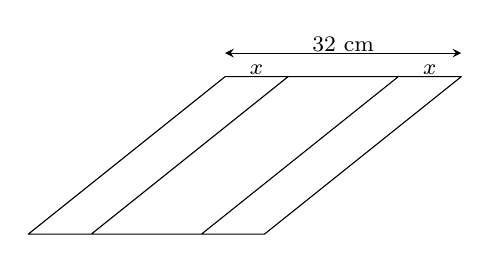
\begin{tikzpicture}[scale=1, font=\footnotesize, line join=round, line cap=round, >=stealth]
	\path
		(0,0) coordinate (A)++(3,0) coordinate (B)++(-2.5,-2) coordinate (C)++(-3,0) coordinate (D)
		(A)++(0.8,0) coordinate (E)++(-2.5,-2) coordinate (F)
		(B)++(-0.8,0) coordinate (G)++(-2.5,-2) coordinate (H)
		(A)++(0,0.3)coordinate (A1)++(3,0) coordinate (A2);
	\draw
		(A)--(B)--(C)--(D)--cycle (E)--(F) (G)--(H)
		(A)--(E)node[above=-1mm, midway]{$x$} (B)--(G)node[midway, above=-1mm]{$x$};
	\draw[<->] (A1)--(A2)node[midway, above=-1mm]{$32$ cm};
	\end{tikzpicture}
	\end{minipage}
	\begin{minipage}{0.5\textwidth}
	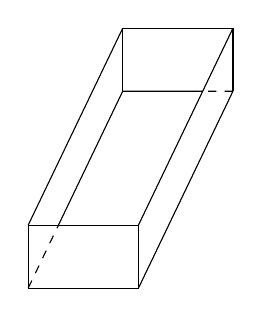
\begin{tikzpicture}
	\path
		(0,0) coordinate (A)++(1.4,0) coordinate (B)++(0,0.8) coordinate (C)++(-1.4,0) coordinate (D)
		(A)++(1.2,2.5)coordinate (A1)++(1.4,0) coordinate (B1)++(0,0.8)coordinate (C1) ++(-1.4,0) coordinate (D1);
	\draw (A)--(B)--(C)--(D)--cycle (A1)--(D1)--(C1)--(B1);
	\foreach \p in {B,C,D} { \draw (\p)--(\p1);}
	\path
		(intersection of A--A1 and C--D) coordinate (A2)
		(intersection of A1--B1 and C--C1) coordinate (B2);
	\draw[dashed] (A)--(A2) (B1)--(B2);
	\draw (A2)--(A1)--(B2);
	\end{tikzpicture}
	\end{minipage}
	\loigiai{
	Bề ngang còn lại của tấm tôn sau khi gấp là $32-2x$ (cm).\\
	Diện tích mặt cắt ngang rãnh nước $S=x(32-2x)=-2x^2+32x$.\\
	Theo giả thiết, $S\geq 120 \Leftrightarrow -2x^2+32x-120\geq 0$.\\
	Ta có $-2x^2+32x-120=0\Leftrightarrow x=6$ hoặc $x=10$.\\
	Lập bảng xét dấu\\
	\centerline{
	\begin{tikzpicture}%
	\tkzTabInit[lgt=4]
		{$x$/0.7, $-2x^2+32x-120$/0.7}
		{$-\infty$, $6$, $10$, $+\infty$}
	\tkzTabLine
		{, - , $0$, +, $0$, -,}
	\end{tikzpicture}
	}\\
	Vậy rãnh dẫn nước đạt yêu cầu khi chiều cao tối thiểu là $6$ cm và chiều cao tối đa là $10$ cm.
	}
	\end{bt}

%% Câu 4
\begin{bt}%[0D7C3-2]%[Dự án đề kiểm tra Toán khối 10 GHKII NH23-24-Dot2-Lê Hữu Kiệt]%[Deso7-CTST]
	Phương trình $2(1-x)\sqrt{x^2+2x-1}=x^2-2x-1$ có các nghiệm dạng $x=a\pm b\sqrt{c}$ trong đó $a\in\mathbb{Z}$, $b$, $c\in\mathbb{N}$. Tính tổng $a+b+c$.
	\loigiai{
	Điều kiện xác định: $x^2+2x-1\geq 0\Leftrightarrow \hoac{&x\leq -1-\sqrt2 \\ &x\geq -1+\sqrt2.}$.\\
	Ta có
	\begin{eqnarray*}
		&& 2(1-x)\sqrt{x^2+2x-1}=x^2-2x-1 \\
		&\Leftrightarrow & x^2-2x-1-2(1-x)\sqrt{x^2+2x-1}=0 \\
		&\Leftrightarrow & (x^2+2x-1)-2(1-x)\sqrt{x^2+2x-1}+(x^2-2x+1)=x^2+2x+1 \\
		&\Leftrightarrow & (1-x-\sqrt{x^2+2x-1})^2=(x+1)^2\\
		&\Leftrightarrow & \hoac{& 1-x-\sqrt{x^2+2x-1}=x+1  \\ & 1-x-\sqrt{x^2+2x-1}=-x-1}\\
		&\Leftrightarrow& \hoac{& \sqrt{x^2+2x-1}=2x \quad\quad(1) \\ &\sqrt{x^2+2x-1}=2. \quad\quad(2)}
	\end{eqnarray*}
	Phương trình $(1)$ tương đương $\heva{&-2x\geq 0 \\ & x^2+2x-1=4x^2} \Leftrightarrow \heva{&x\geq 0 \\ &3x^2-2x+1=0} \Leftrightarrow x\in\varnothing$.\\
	Phương trình $(2)$ tương đương $x^2+2x-1=4 \Leftrightarrow x^2+2x-5=0 \Leftrightarrow x=-1\pm\sqrt6$.\\
	Suy ra $a=-1$, $b=1$, $c=6$.\\
	Vậy $a+b+c=-1+1+6=6$.
	}
	\end{bt}

%% Câu 5
\begin{bt}%[0H9N1-4]%[Dự án đề kiểm tra Toán khối 10 GHKII NH23-24-Dot2-Lê Hữu Kiệt]%[Deso7-CTST]
	Cho $A(2;-4)$, $B(6;0)$, $C(m;4)$. Định $m$ để $A$, $B$, $C$ thẳng hàng.
	\loigiai{
	Ta có $\vec{AB}=(4;4)$, $\vec{AC}=(m-2;8)$.\\
	Để $A$, $B$, $C$ thẳng hàng khi và chỉ khi $\vec{AB}$, $\vec{AC}$ cùng phương, tương đương
	$$\dfrac{m-2}{4}=\dfrac{8}{4}\Leftrightarrow m=10.$$
	Vậy $m=10$ thì $A$, $B$, $C$ thẳng hàng.
	}
	\end{bt}

%% Câu 6
\begin{bt}%[0H9V1-3]%[Dự án đề kiểm tra Toán khối 10 GHKII NH23-24-Dot2-Lê Hữu Kiệt]%[Deso7-CTST]
	Cho $\triangle ABC$ có trung điểm cạnh $BC$ là $M(-1;-1)$, $AB\colon x+y-2=0$, $AC\colon 2x+6y+3=0$. Tìm tọa độ ba điểm $A$, $B$, $C$.
	\loigiai{
	Ta có $A=AB\cap AC$, suy ra tọa độ điểm $A$ là nghiệm của hệ phương trình
	$$\heva{&x+y-2=0 \\ &2x+6y+3=0} \Leftrightarrow\heva{&x=\dfrac{15}{4} \\ &y=-\dfrac{7}{4}.}$$
	Vậy $A\left(\dfrac{15}{4};-\dfrac{7}{4}\right)$.\\
	Ta có $B\in AB$, suy ra $B(x_B;-x_B+2)$, $C\in AC$, suy ra $C\left(x_C;\dfrac{-2x_C-3}{6}\right)$.\\
	Do $M$ là trung điểm của $BC$ nên
	$$\heva{&x_B+x_C=2x_M \\ &y_B+y_C=2y_M} \Leftrightarrow \heva{&x_B+x_C=-2 \\ &-x_B+2+\dfrac{-2x_C-3}{6}=-2} \Leftrightarrow \heva{&x_B+x_C=-2 \\ &-6x_B-2x_C=-21} \Leftrightarrow \heva{&x_B=\dfrac{25}{4} \\&x_C=-\dfrac{33}{4}.}$$
	Vậy $B\left(\dfrac{25}{4};-\dfrac{17}{4}\right)$, $C\left(-\dfrac{33}{4};\dfrac{9}{4}\right)$.
	}
	\end{bt}
%%%%%%%%%% Hết phần tự luận %%%%%%%%%%
